\subsection{Overview}

\begin{figure}[htbp]
  \centering
  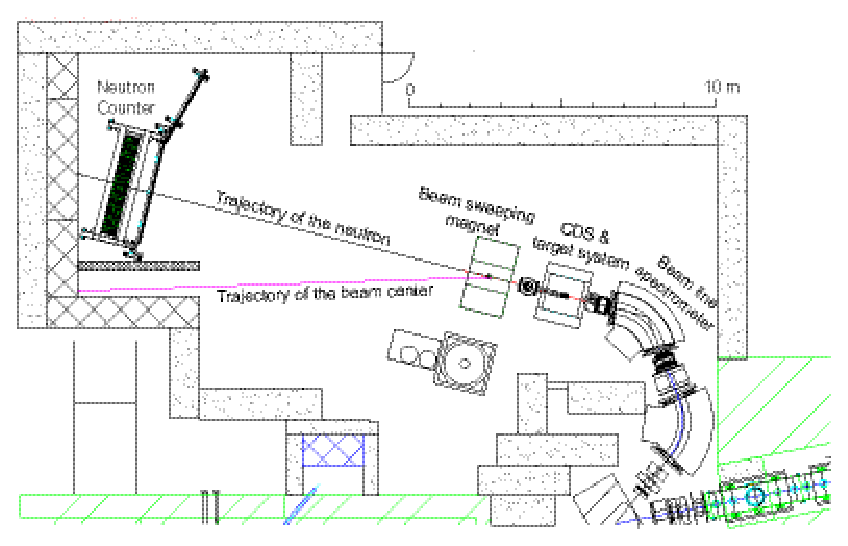
\includegraphics[width=8cm]{pic/experiment/hall.eps}
  \caption{
    Schematic view of the experimental hall at the K1.8BR.
  }
  \label{fig:ex_hall}
\end{figure}


This section describes the beamline detector systems.
Fig.\ref{fig:ex_hall} shows the schematic view of experimental area in which install detectors described in this section.
The Aerogel Cherenkov (AC) counter for identifying kaon beams is described first.
Next, the hodoscope detectors, BHD and T0, are described to confirm that the beam is a kaon beam by TOF (time of flight) method.
The beam momentum analysis is performed by using a D5 magnet placed upstream of the T0 detector as a spectrometer.
Multiple wire drift chambers (MWDC) named BLC1 and BLC2 are placed upstream and downstream of the D5 magnet respectively, and the beam momentum is reconstructed from these trajectories.
The FF beam trajectory is measured by the BPC of the MWDC, which is located just upstream of the target.
The beam definition counter (DEF) are mounted to the target vacumm chamber to reduce the trigger signal, which can cause a reduction in DAQ efficiency.
Also, BPD is briefly described, which is the counter placed upstream of BPC, although this is not used in the analysis described in this article.
